% ------------------------------------------------------------%
% 2015-2021 - Emerson Ribeiro de Mello <mello@ifsc.edu.br>
% ------------------------------------------------------------%
% Sets aspect ratio to 4:3, and frame size to 128 mm by 96 mm
\documentclass[aspectratio=169]{beamer}
% Sets aspect ratio to 16:9, and frame size to 160 mm by 90 mm.
% \documentclass[aspectratio=169]{beamer}
% Sets aspect ratio to 16:10, and frame size to 160 mm by 100 mm.
% \documentclass[aspectratio=1610]{beamer}
\usepackage[dvipsnames]{xcolor}
\usepackage{colortbl}
\usepackage{makecell}
\usepackage{multicol}
\usepackage{pifont}

\definecolor{DarkCyan}{HTML}{119DA4}
\definecolor{Asparagus}{HTML}{6DA34D}
\definecolor{CambridgeBlue}{HTML}{8FBC94}
\definecolor{TeaGreen}{HTML}{C5E99B}
\definecolor{Saphire}{HTML}{4059AD}



% -------------------------------------------------%
%  Package options
% -------------------------------------------------%
%  002625, EEE5E9, 0D1821, ADF7B6, B6C454
% textbgcolor   - frametitle background color. default: 0d4f4d
% textfgcolor   - frametitle foreground color. default: ffffff
% slidebgcolor  - slide background color. default: eef1ec
% slidefgcolor  - slide text foreground color. default: 000000
% authorfgcolor - author, institute and date color. default: 000000
% itemsep - space between items (itemize, enumerate). default: 7pt
\usepackage[textbgcolor=344966,textfgcolor=ffffff,slidebgcolor=EEE5E9,itemsep=7pt]{../0-ifscyan-modelo/beamerthemeifscyan}
% -------------------------------------------------%

% A good place to get some colors
% https://material.io/resources/color/#!/?view.left=0&view.right=0&primary.color=0d4f4d
% cyan: #0D4F4D, light: #417b79,  dark: #002625
% IFSC green: normal: #32A041, light: #69d26f, dark: #007013
% IFSC red: normal: #C8191E, light: #ff5747, dark: #8f0000 
% Other colors for textbgcolor
% purple 4527a0, blue 0d47a1, grey 546e7a, redwine 880e4f, brown 6d4c41, yelllow (bg=#fbc02d, fg=000000)

% Logo
\pgfdeclareimage[height=.3\paperheight]{ifpilogo}{../0-ifscyan-modelo/figs/Logo-IFPI-Vertical.png}

\AtBeginSection[]{
  \begin{frame}
  \vfill
  \centering
  \begin{beamercolorbox}[sep=8pt,center,shadow=true,rounded=true]{title}
    \usebeamerfont{title}\insertsectionhead\par%
  \end{beamercolorbox}
  \vfill
  \end{frame}
}

% -------------------------------------------------%
%              Título 
% -------------------------------------------------%
\title{Matemática Computacional}
\subtitle{Conjuntos - Exercícios}
\author{Prof. Rogério Figueredo de Sousa}
\institute{%
\href{rogerio.sousa@ifpi.edu.br}{rogerio.sousa@ifpi.edu.br}%
}%
\date{22/08/2024}
% -------------------------------------------------%

% -------------------------------------------------%
%  Início do documento 
% -------------------------------------------------%
\begin{document}

\begin{frame}[plain]
    \titlepage
\end{frame}

%\begin{frame}[plain, noframenumbering]{Licenciamento}
%    \licenciamentoLivre
%\end{frame}

%\begin{frame}[plain, noframenumbering]{Sumário}
%   \tableofcontents
%\end{frame}


\jsonp
\lstset{
    numbers=none,
    escapeinside={\%*}{*)},
}

%12
\begin{frame}{Conjuntos - Exercícios}
    Exercício 1: Julgue se os conjuntos são finitos ou infinitos:
    \vspace{4mm}
\begin{enumerate}
    \item Conjunto das letras do alfabeto;
    \item $P = \{y | y = 2x ~ e ~ x \in \mathbb{N} \}$
    \item $M = \{x \in \mathbb{N} | x > 0 ~ e ~ x < 6\}$
    \item O conjunto do números naturais.
\end{enumerate}    
\end{frame}

%13
\begin{frame}{Conjuntos - Exercícios}
    Exercício 2: Descreva cada um dos conjuntos a seguir listando seus elementos:
    \vspace{4mm}
\begin{enumerate}
    \item $A=\{x|x ~ \acute{e} ~ um ~ inteiro ~ e ~ 3 < x < 8\}$
    \item $B=\{x|x ~ \acute{e} ~ um ~ m\hat{e}s ~ com ~ exatamente ~ 30 ~ dias\}$
    \item $C=\{x|x ~ \acute{e} ~ a ~ capital ~ do ~ Brasil\}$
    \item $D=\{x|(\exists y)(y \in \{0,1,2\} ~ e ~ x = y^3)\}$
    \item $E=\{x|x \in \mathbb{N} ~ e ~ (\exists y)(y \in \mathbb{N} ~ e ~ x \leq y)\}$
    \item $F=\{x|x \in \mathbb{N} ~ e ~ (\forall y)(y \in \mathbb{N} ~ \rightarrow ~ x \leq y)\}$
    \item $A = \{x | x \in \mathbb{N} ~ e ~ (\forall y)(y \in \{2, 3, 4, 5\}) \rightarrow x \geq y\}.$
    \item $B = \{x | (\exists y)(\exists z)(y \in \{1,2\} ~ e ~ z \in \{2,3\} ~ e ~ x=y+z)\}$
\end{enumerate}    
\end{frame}

%14
\begin{frame}{Conjuntos - Exercícios}
    Exercício 3: Descreva cada um dos conjuntos a seguir através de uma relação de recorrência.
    \vspace{4mm}
\begin{enumerate}
    \item $A=\{2,4,16,256,...\}$
    \item $B=\{1,4,9,16,...\}$
    \item $C=\{1,3,9,27,...\}$
\end{enumerate}    
\end{frame}

\begin{frame}{subconjuntos}
    \textbf{Exercício 4:}
    \vspace{4mm}

    Sejam $A = \{x | x \in \mathbb{N} ~ e ~ x \geq 5\}$, $B = \{10, 12, 16, 20\}$ e $C = \{x | (\exists y)(y \in \mathbb{N} ~ e ~ x = 2y)\}$

    Quais das proposições abaixo são verdadeiras:
    
    \begin{multicols}{2}
        \begin{itemize}
            \item $B \subseteq C$
            \item $B \subset A$
            \item $A \subseteq C$
            \item $26 \in C$
            \item $\{11, 12, 13\} \subseteq A$
            \item $\{11, 12, 13\} \subset C$
            \item $\{12\} \in B$
            \item $\{12\} \subseteq B$
            \item $\{x | x \in \mathbb{N} ~ e ~ x < 20\} \nsubseteq B$
            \item $5 \subseteq A$
            \item $\{\emptyset\} \subseteq B$
            \item $\emptyset \notin A$
        \end{itemize}
    \end{multicols}
\end{frame}

%20
\begin{frame}{subconjuntos}
    \textbf{Exercício 5:}
    \vspace{4mm}
    
    Sejam: 
    
    \[A = \{x | x \in \mathbb{R} ~ e ~ x^2 - 4x + 3 = 0\}\]

e

    \[B = \{x | x \in \mathbb{N} ~ e ~ 1 \leq x \leq 4\}\]
    \vspace{4mm}
Prove que $A \subset B.$

\end{frame}

%21
\begin{frame}{subconjuntos}
    \textbf{ Exercício 6:} Sejam

    \[ A = \{x|x \in \mathbb{N} ~ e ~ x^2 < 15\} \]
    e
    
    \[ B = \{x|x \in \mathbb{N} ~ e ~ 2x < 7 \} \]

    Prove que $A = B.$
 
 \end{frame}

%23
\begin{frame}{subconjuntos}
    \textbf{Exercício 7:} 
    
    \begin{enumerate}
        \item Para $A=\{1,2,3\}$, qual é o $\wp(A)$?
        \vspace{4mm}
        \item Se S tem \textit{n} elementos, então $\wp(A)$ tem quantos elementos?
    \end{enumerate}
        
\end{frame}

%25
\begin{frame}{subconjuntos}
    \textbf{Exercício 8: }
    \noindent
Sobre o conjunto $A = \{1, 2, 3, 4\}$, considere as afirmativas a seguir.

\begin{enumerate}
    \item $\mathcal{P}(A) = \{\emptyset, \{2, 3, 4\}\}$ é uma partição de $A$.
    \item $\mathcal{P}(A) = \{\emptyset, \{1, 2, 3\}, \{3, 4\}\}$ é uma partição de $A$.
    \item $\mathcal{P}(A) = \{\{1, 2\}, \{3, 4\}\}$ é uma partição de $A$.
    \item $\mathcal{P}(A) = \{\{1\}, \{2\}, \{3\}, \{4\}\}$ é uma partição de $A$.
\end{enumerate}

\noindent
Assinale a alternativa correta.

\begin{enumerate}[a)]
    \item Somente as afirmativas I e II são corretas;
    \item Somente as afirmativas I e IV são corretas;
    \item Somente as afirmativas III e IV são corretas;
    \item Somente as afirmativas I, II e III são corretas;
    \item Somente as afirmativas II, III e IV são corretas;
\end{enumerate}
\end{frame}

\begin{frame}{Exercícios}

    \textbf{Exercício 9: }
    Sejam
\[ A = \{x | x ~ \acute{e} ~ um ~ inteiro ~ n\tilde{a}o - negativo ~ par \} \]
\[ B = \{x | (\exists y) (y \in \mathbb{N} ~ e ~ x = 2y + 1 )\} \]
\[ C = \{x|(\exists y)(y \in \mathbb{N} ~ e ~ x = 4y)\} \]

Julgue a veracidade de cada alternativa:

\begin{enumerate}[a)]
    \item $A \cup B$
    \item $A = B$
    \item $ C \subset A$
    \item $A \cup C$
    \item $A - C = \{x|(\exists y)(y \in \mathbb{N} ~ e ~ x = 4y + 2)\}$
\end{enumerate}
\end{frame}


\begin{frame}{Exercícios}

    \textbf{Exercício 10: }

    Sejam
\[ A = \{1,2,3,5,10\} \]
\[ B = \{2,4,7,8,9\} \]
\[ C = \{5,8,10\} \]

Se $S=\{1,2,3,4,5,6,7,8,9,10\}$, encontre:

\begin{enumerate}[a)]   
    \item $|A| + |B|$
    \item $A \cup B$
    \item $A - C$
    \item $B \cap (A \cup C)$
    \item $\overline{C}$
\end{enumerate}
\end{frame}


\begin{frame}{Exercícios}
    \textbf{Exercício 11: }
\begin{figure}
    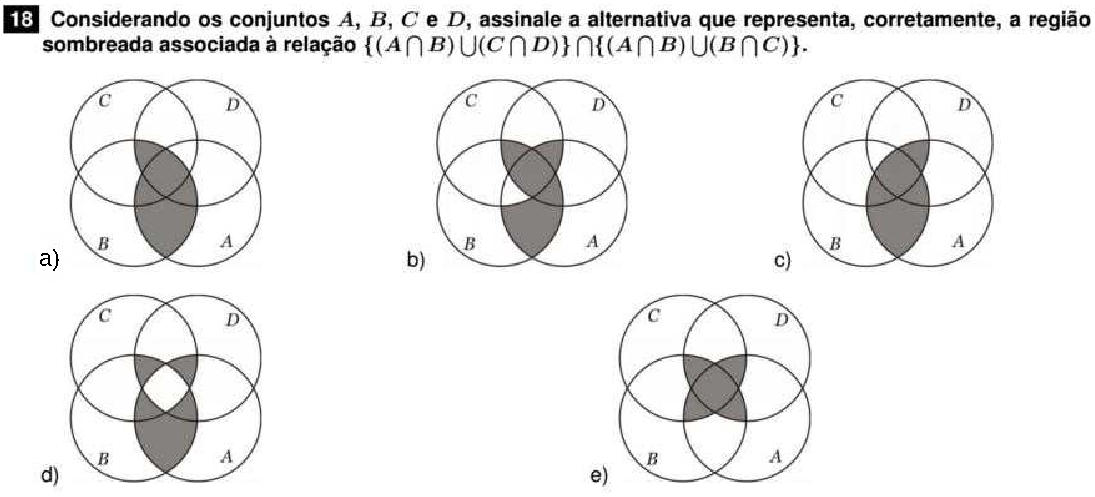
\includegraphics[width=0.9\textwidth]{./figs/poscomp18-cropped.pdf}
\end{figure}
\end{frame}

\begin{frame}{Identidades Básicas}
    \begin{itemize}
        \item \textbf{Exercício 12:} Usando as identidades básicas, prove a identidade:

            \[
            [C \cap (A \cup B)] \cup \left[(A \cup B) \cap \overline{C}\right] = A \cup B
            \]

            \begin{center}
                (A, B e C são subconjuntos arbitrários de $S$.)
            \end{center}
        \item \textbf{Ex. 2} Enuncie a identidade dual do exemplo anterior.

        \item \textbf{Ex. 3} Usando as identidades básicas, prove a identidade: 
        
        \[
        (A \cup B) \cap (A \cup \overline{B}) = A
        \]
    \end{itemize}
\end{frame}

\begin{frame}{Exercícios}

    \textbf{Exercícios 13 e 14:}

\begin{itemize}
    \item Liste os elementos dos seguintes conjuntos:
    \begin{itemize}
        \item $\{ x ~ | ~ x ~ \acute{e} ~ um ~ n\acute{u}mero ~ real ~ e ~ x^2 = 1 \}$
        \item $\{ x ~ | ~ x \in \mathbb{Z} ~ e ~ |x| < 4 \}$ ($|x|$ denota a função valor absoluto)
        \item $\{x ~ | ~ x ~ \acute{e} ~ m\acute{u}ltiplo ~ de ~ 4 \}$
    \end{itemize}

    \item Descreva cada um dos seguintes conjuntos, atribuindo-lhes uma propriedade específica:
    \begin{itemize}
        \item $S = \{1, 4, 9, 16\}$
        \item $S = \{2, 3, 5, 7, 11, 13, . . . \}$
        \item $S = \{0, 1, 10, 11, 100, 101, 110, 111, 1000, \dots \}$
    \end{itemize}
\end{itemize}
\end{frame}

\begin{frame}{Exercícios}
    \textbf{Exercícios 15 e 16}
\begin{itemize}
    \item Sejam os conjuntos: $A = \{x ~ | ~ x ~ \acute{e} ~ par ~ positivo ~ e ~ x < 15\}$, $B = \{x \in N ~ | ~ x < 15\}$ e $C = \{x ~ | ~ x < 15 ~ e ~ x ~ \acute{e} ~ primo \}$. Insira os elementos correspondentes no diagrama de Euler-Venn:
    \item Faça um diagrama de Euler-Venn que simbolize a seguinte situação: A, B, C, D são conjuntos não vazios e $D \subset C \subset B \subset A$.
\end{itemize}
\end{frame}

\begin{frame}{Exercícios}
    \textbf{Exercício 17}
\begin{itemize}
    \item Sejam $U ~ (universo) ~ = ~ \{n \in \mathbb{N} ~ | ~ 0 \leq n \leq 9\}$, $A = \{1, 2, 3, 4\}$, $B = \{x ~ \in ~ \mathbb{R} | (x - 1) (x - 3)^3 = 0\}$ e $C = \{n ~ \in ~ \mathbb{N} | ~ n ~ \acute{e} ~ \acute{i}mpar \}$. Determine:
    \begin{enumerate}
        \item $A \cup B$
        \item $A \cap (B \cup C)$
        \item $C - A$
        \item $ \overline{A} \cup C$
        \item a cardinalidade de A, B e C
    \end{enumerate}
\end{itemize}

\end{frame}



\begin{frame}{Exercícios}
    \textbf{Exercício 18}

\begin{itemize}
    \item Sejam os conjuntos $A = \{a, b, c\}$, $B = \{x, y\}$ e $C = \{0, 1\}$. Encontre os seguintes produtos cartesianos:
    \begin{itemize}
        \item $A \times B$
        \item $C \times A$
    \end{itemize}

\end{itemize}

\end{frame}

\begin{frame}{Exercícios}

    \textbf{Exercício 19}


\begin{itemize}
    \item A, B e C são subconjuntos de um conjunto S. Prove as identidades a seguir usando as identidades básicas envolvendo conjuntos.
    \begin{itemize}
        \item $(A \cup B) \cap (A \cup \overline{B}) = A$
        \item $A \cap (B \cap \overline{A}) = B \cap A$
    \end{itemize}
\end{itemize}
\end{frame}


\end{document}